
\tjzspis{Człowiek ukryty w genomie} %tytuł do spisu treści
\tjztyt{Człowiek ukryty w genomie} %tytuł odcinka 


{%\advance\baselineskip by-.1pt\advance\parskip by-1pt
W połowie lutego 2001 roku amerykański noblista, mikrobiolog, David Baltimore we wstępniaku do magazynu Nature wyznał: ,,Widziałem wiele ekscytujących odkryć z biologii w ciągu ostatnich 40 lat, jednak czułem ciarki na plecach, gdy czytałem artykuł opisujący zarys naszego genomu''. 

Zapowiadał w ten sposób pracę, w której konsorcjum Human Genome Project opisywało wstępne wyniki sekwencjonowania ludzkiego DNA. Start projektu w 1990 roku ogłosił sam James Watson, który porównał zadanie rozszyfrowania informacji ukrytej w ludzkim DNA do misji lądowania człowieka na Księżycu. 

Przez kilkanaście lat napięcie rosło, oczekiwania były olbrzymie, miało się przecież okazać, jak na poziomie cząsteczek realizowane jest powstanie człowieka. Jednym z ważniejszych parametrów, o którym dyskutowano, była liczba genów
% sprawiających, że jesteśmy ludźmi.
zakodowanych w~naszym DNA.
Wiadomo było już sporo o liczbie genów u innych organizmów.  np. bakteria \textit{Escherichia coli} ma ich około 4 tysięcy, maleńka roślina, rzodkiewnik pospolity -- 25,5 tysiąca, a mierzący 1 mm nicień \textit{Caenorhabditis elegans} około 20 tysięcy. 

Dziś mogę fantazjować, że może tuż po ciarkach u noblisty pojawiły się  krople potu, bowiem wstępny wynik był zadziwiający: ogłoszono, że genom ludzki koduje między 20 tysięcy a 30 tysięcy genów. Ta  skromna liczba mogła podsuwać wątpliwości, czy w opisie funkcjonowania żywych komórek nie popełniono fundamentalnego błędu?

Tu muszę doprecyzować, co w tej wyliczance oznacza słowo ,,gen''. Definiowano go jako fragment DNA, w którym zakodowana jest informacja o budowie białka. Białko zaś to cząsteczka, która się składa z łańcucha nie mniej niż 100 aminokwasów. 

Analiza całego genomu ludzkiego wykazała, że sekwencje, które kodują białka, to jedynie 1 do 2\% całości. Powstało zatem pytanie: co znajduje się w pozostałej ,,ciemnej materii'' (\textit{dark genome})?

Po ponad 20 latach wiemy  więcej, choć wiele pozostaje do wyjaśnienia. 

Najwięcej jest reliktów z przeszłości, fragmentów samorzutnie kopiujących się, pradawnych wirusów i innych aktywnych elementów, które są skutkiem procesów zachodzących w DNA. Dużą część genomu stanowią sekwencje kodujące różne typy RNA, cząsteczek, które mają fundamentalne funkcje dla życia komórki. Biorą udział w tworzeniu struktur niezbędnych do produkcji białek. Wiele z nich, w tym bardzo krótkie, reguluje działanie genów: ilość produkowanych białek, to, jak długo są produkowane i jak szybko są degradowane. Nie można też zapomnieć o fragmentach pełniących funkcje strukturalne -- dzięki niektórym bardzo długie cząsteczki DNA mogą być pakowane do struktur odpornych na uszkodzenia mechaniczne, co jest krytyczne w trakcie podziałów komórkowych; inne sprawiają, że cząsteczki DNA nie ulegają skracaniu; a dzięki innym DNA może być duplikowany.  

Czas eksploracji jeszcze się nie skończył. John Prensner, neuroonkolog dziecięcy z~Bostonu po bezskutecznych,
% postanowił sprawdzić, co ukrywa się w zakamarkach genomu, ponieważ prowadzone przez niego
poszukiwaniach genów związanych z nowotworami u dzieci
wrócił do analizy genomu, zmieniając kryteria wyszukiwania.
% okazywały się bezskuteczne.
Podstawą były
sporadyczne
% pojawiające się od jakiegoś czasu
informacje o istnieniu w komórkach cząsteczek będących łańcuchami aminokwasów krótszych niż 100. Prensner przyznaje, że było mu trudno uzyskać finasowanie dla badań nad takimi minibiałkami, gdyż uznawano je dotąd za komórkowe ,,śmieci'', szybko ulegające degradacji. Udało mu się jednak zgromadzić międzynarodowe grono, które podjęło się poszukiwania minibiałek. Dzięki analizie wielu prac badawczych i baz danych kanoniczna definicja ,,białko to więcej niż 100 aminokwasów'' została w końcu podważona. 

Okazało się, że spośród 7264 sekwencji, które mogłyby kodować minibiałka, około jedna czwarta  jest aktywna, dzięki czemu powstaje około 3000~różnych minibiałek (jedna sekwencja DNA może kodować więcej niż jedno~białko). \marg{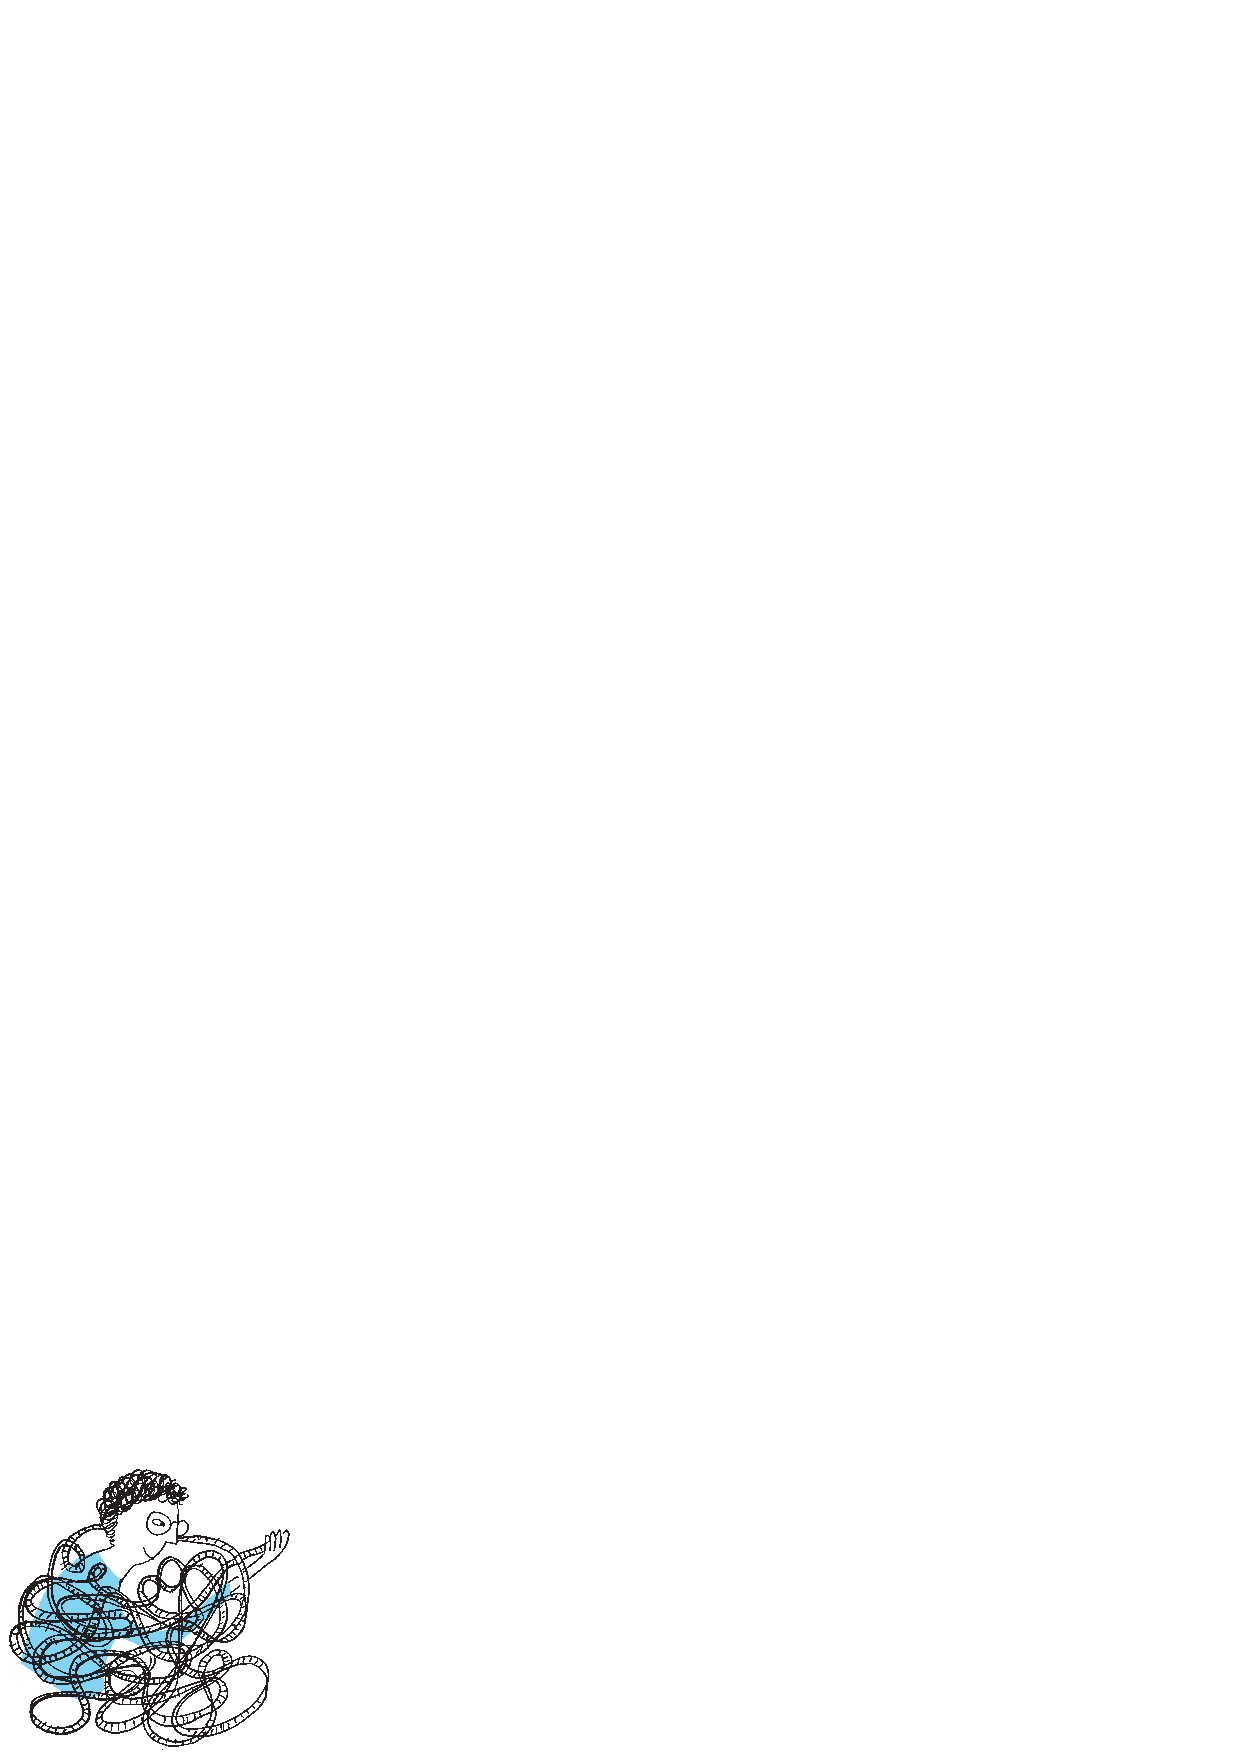
\includegraphics{art/202501_kol10}}

Jedno z nich, ASDURF, jest na przykład produkowane w nadmiarze w komórkach rdzeniaka zarodkowego, trudnego do zdiagnozowania nowotworu dziecięcego. Jego nadprodukcja wydłuża czas życia komórek nowotworowych. Inne badania wskazują na rolę mikrobiałek w rozwoju otyłości, raka trzustki i w chorobach metabolicznych.

Co zatem stanowi esencję ,,człowieka'' na poziomie cząsteczek? Jako jedyny gatunek, który jest w stanie analizować własny genom, musimy wciąż zachować pokorę dla złożoności rozwiązań natury i cierpliwie szukać dalszych odpowiedzi. Bo przecież wiadomo było, że to nie może być proste{\dots}


}

\medskip
\rightline{\large\it Marta FIKUS-KRYŃSKA}

\hspace*{-5.5cm}\vrule height5pt depth-4.5pt width18cm

\normalsize

\endinput
\marg{Kiedyś uważano, że za każdą cechę odpowiada jeden gen. Czyli jest np. gen jasnych włosów, brązowych włosów, czarnych włosów, jest gen dobrego węchu czy też dobrego wzroku itp. Dziś wiemy, że tak zwanych cech jednogenowych jest bardzo, bardzo niewiele, a większość z naszych cech determinuje kilkaset genów!}
